 \documentclass{report}
 
\usepackage[utf8]{inputenc} 
\usepackage[T1]{fontenc}      
\usepackage[top=2.0cm, bottom=3cm, left=3.0cm, right=3.0cm]{geometry}
\usepackage{graphicx}
\usepackage{wrapfig}
\usepackage{amsmath,esint}
\usepackage{amssymb}
\graphicspath{{figures/}{../figures}}

\newcommand*\dif{\mathop{}\!\mathrm{d}}
\newcommand*\diver{\mathop{}\!\mathrm{div}}
\newcommand*\grad{\mathop{}\!\mathrm{grad}}

\begin{document}

\section*{Question de cours}

\subsection*{Premier principe}

\textit{A tout système thermodynamique fermé, est associé une équation d'état $E$ appelée énergie. Au cours d'une variation quelconque, la variation de $E$ est égale à l'énergie reçue.}

Pour la plupart des transformations étudiées, $\Delta E = \Delta E_{méca}+\Delta U =  \Delta U $ car la variation d'énergie mécanique est faible durant la transformation (pour un gaz notamment).

Le premier principe s'exprime :
\begin{equation}
	\Delta U = W+Q
\end{equation}
ou :
\begin{equation}
	d U = \delta W+ \delta Q
\end{equation}
Ce principe est extrêmement fondamental car il représente la conservation de l'énergie en physique.
 
\section*{Machine de Carnot}

\begin{itemize}

	\item[0 -] Le cycle est moteur, il est décrit "en tournant" dans le sens des aiguilles d'une montre dnas le diagramme de Clapeyron. L'intégrale $W=-\oint P\dif V<0$ est négative donc le travaile st bien évacué à l'extérieur.

	\item[1 -] On trouve les expressions grâce à l'expression du travail $W$ et au premier principe de la thermodynamique. Le point "difficile" est le calcul du travail pour une transformation adiabatique. Il faut utiliser la loi de Laplace : 

\begin{align*}
	\delta W = -\int_B^C P\dif V &= -cste\int_B^C \frac{\dif V}{V^{\gamma}}\\
	&=-cste\frac{V_C^{1-k}-V_B^{1-k}}{1-k}\\
	&=\frac{P_CV_C-P_BV_B}{\gamma-1}\\
	&= \frac{nR}{\gamma-1}(T_c-T_f)
\end{align*}

Le tableau des différentes transformations est alors :

\begin{center}
\begin{tabular}{|p{2,5cm}|p{3cm}|p{3cm}|p{3cm}|}
\hline
Transformation & $\Delta U$ & $W$ & $Q$ \\
\hline
$A\rightarrow B$ & 0  & $nRT_f\ln\left(\frac{V_A}{V_B} \right)$  & $-nRT_f\ln\left(\frac{V_A}{V_B} \right)$  \\
\hline
$B\rightarrow C$ & $\frac{nR}{\gamma-1}(T_c-T_f)$ & $\frac{nR}{\gamma-1}(T_c-T_f)$ & 0  \\
\hline
$C\rightarrow D$ & 0  & $-nRT_c\ln\left(\frac{V_D}{V_C} \right)$  & $ nRT_c\ln\left(\frac{V_D}{V_C} \right)$ \\
\hline
$D\rightarrow A$ & $\frac{nR}{\gamma-1}(T_f-T_c)$ & $\frac{nR}{\gamma-1}(T_f-T_c)$ & 0 \\
\hline
\end{tabular}
\end{center}

\item[2-]  Le rendement est $\eta=-W/Q_c$. La source chaude est ici :

\begin{align*}
	Q_c&=Q_{C\rightarrow D}\\
	&=nRT_c\ln\left(\frac{V_D}{V_C} \right)\\
\end{align*}		
Et le travail :	
\begin{align*}
	W&=\sum_i W_i\\
	&=nRT_f\ln\left(\frac{V_A}{V_B} \right)-nRT_c\ln\left(\frac{V_D}{V_C} \right)\\
	&=nR(T_f - T_c)\ln\left(\frac{V_A}{V_B} \right)\\
\end{align*}		
car on a $V_A/V_B=V_D/V_C$ avec la loi de Laplace $TV^{\gamma-1}=cste$.
On trouve alors :
\begin{align*}
	\eta=\frac{T_f-T_c}{T_c}=1-\frac{T_f}{T_c}
\end{align*}
C'est le rendement de Carnot : c'est normal, c'est un cycle de Carnot !

\end{itemize}

\subsection*{Cycle de Beau de Rochas}

\begin{itemize}

	\item[0 -] Il faut utiliser la loi de Laplace : 

\begin{align*}
	\delta W = -\int_i^f P\dif V &= -cste\int_i^f \frac{\dif V}{V^{\gamma}}\\
	&=-cste\frac{V_f^{1-k}-V_i^{1-k}}{1-k}\\
	&=\frac{P_fV_f-P_iV_i}{\gamma-1}\\
	&= \frac{nR}{\gamma-1}(T_f-T_i)
\end{align*}

	\item[1 - ] On utilise le résultat précédent pour les transformations $A\rightarrow B$ et $D\rightarrow A$. Pour les transformations isochores, on calcule $\Delta U$ tout simplement pour l'échauffement d'un gaz.

\begin{center}
\begin{tabular}{|p{2,5cm}|p{3cm}|p{3cm}|p{3cm}|}
\hline
Transformation & $\Delta U$ & $W$ & $Q$ \\
\hline
$A\rightarrow B$ & $\frac{nR}{\gamma-1}(T_B-T_A)$  & $\frac{nR}{\gamma-1}(T_B-T_A)$  & 0  \\
\hline
$B\rightarrow C$ & $\frac{nR}{\gamma-1}(T_C-T_B)$ & 0 & $Q_c=\frac{nR}{\gamma-1}(T_C-T_B)$  \\
\hline
$C\rightarrow D$ & $\frac{nR}{\gamma-1}(T_D-T_C)$  & $\frac{nR}{\gamma-1}(T_D-T_C)$ & 0 \\
\hline
$D\rightarrow A$ & $\frac{nR}{\gamma-1}(T_A-T_D)$ & 0 & $Q_f=\frac{nR}{\gamma-1}(T_A-T_D)$ \\
\hline
\end{tabular}
\end{center}

\item[2 -] Pour calculer le rendement, il faut expliciter la quantité de chaleur issue de la source chaude : il s'agit de $Q_{AB}$, car on augmente la pression à volume constant, c'est-à-dire qu'on apporte de la chaleur. Ici, elle est apportée par l'explosion de l'essence. Le travail, quant à lui, s'écrit :

\begin{align*}
	W &= -\frac{nR}{\gamma-1}(T_B-T_A+T_D-T_C)\\
	&=-\frac{nR}{\gamma-1}(T_D-T_A) + Q_c
\end{align*}

Il reste à déterminer $T_D$ par rapport à $T_A$. Pour cela, on détermine la température à chaque transformation :
\begin{itemize}
	\item[$A\rightarrow B$ :] $T_B=a^{\gamma-1}T_A$ car compression adabatique en utilisant $TV^{\gamma-1}=cste$.
	\item[$B\rightarrow C$ :] $T_C=\frac{nR}{\gamma-1}Q_c + T_B$, d'après le premier principe : on échauffe le gaz en lui apportant $Q_c$.
	\item[$C\rightarrow D$ :] $T_D=T_C/a^{\gamma-1}$ car compression adabatique.
\end{itemize}

On a donc :
\begin{align*}
	T_D = \frac{\gamma-1}{a^{\gamma-1}nR}Q_c+T_f
\end{align*}

Donc $W=Q_c\left( 1-\frac{1}{a^{\gamma-1}}\right) $ et alors :
\begin{align*}
	\eta= 1-\frac{1}{a^{\gamma-1}}
\end{align*}

	\item[3 -] Pour comparer avec le rendement de Carnot $\eta_C=1-T_f/T_c$, il faut expliciter les températures de la source chaude $T_c$ et froide $T_f$. La température de la source chaude est à priori $T_C$ car le gaz est au maximum de sa température en $C$. En effet, comme la transformation $C\longrightarrow D$ est réversible, elle est supposée très lente, donc on peut supposer que le gaz s'est thermalisé à la température de la source chaude en $C$. 
	
	A ce moment là :
	\begin{align*}
		\eta_C&=1-\frac{T_A}{T_C}\\
		&=1-\frac{T_A}{\frac{\gamma-1}{nR}Q_c+a^{\gamma-1}T_A}\\
		&=1-\frac{1}{\frac{\gamma-1}{nRT_A}Q_c+a^{\gamma-1}}\\
		&>1-\frac{1}{a^{\gamma-1}} = \eta
	\end{align*}

On retrouve bien le fait que le rendement de Carnot est supérieur.

\end{itemize}

\section*{Exercice 2}

\begin{itemize}

	\item[•] Démonstration de la détente de Joule Thomson. On considère une tranche de $dn$ moles entrant en $x=x_1$ à l'instant $t$. Elle est caractérisée par $U_1$, $T_1$, $P_1$, $H_1$ et $v_1$. 
	
\begin{figure}[!h]

\centering
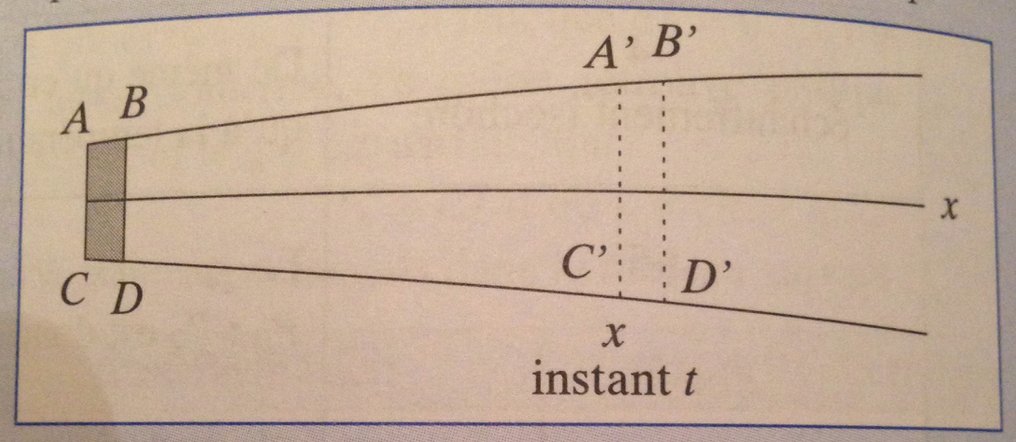
\includegraphics[width=0.4\linewidth]{tuyere1.png}

\end{figure}	

A l'instant $t+\Delta t$, elle est à l'abscisse $x$. Elle est caractérisée par $U(x)$, $T(x)$, $P(x)$, $H(x)$ et $v(x)$. 
	
\begin{figure}[!h]
\centering
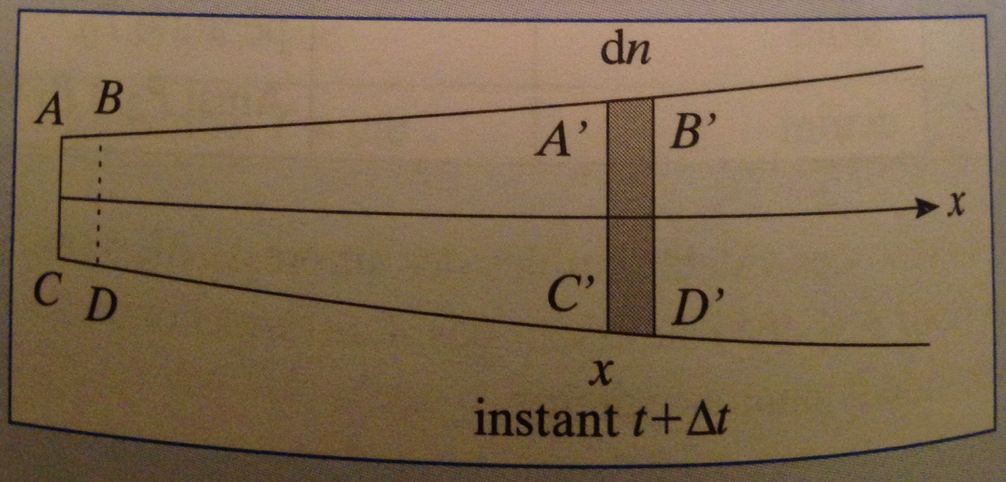
\includegraphics[width=0.4\linewidth]{tuyere2.png}
\end{figure}	

On considère la tranche de gaz $ACA'C'$ à l'instant $t$. A l'instant $t'>t$, elle correspond à la tranche $BDB'D'$, comme le système est en régme permanent. 

On applique le premier principe à la tranche $ACA'C'$. $Q=0$ comme les parois sont adiabatiques. 
Il reçoit en $x=x_1$ un travail $V_{ABCD}P_1$ et en $x$ un travail $V_{A'B'C'D'}P(x)$.

Le premier principe s'écrit alors :
\begin{equation}
	E_{c,BDB'D'} + U_{BDB'D'} - E_{c,ACA'C'} - U_{ACA'C'} = -V_{A'B'C'D'}P(x)+V_{ABCD}P_1
\end{equation}

Comme la partie centrale $BDA'C'$ reste complètement inchangée entre $t$ et $t'$, on a (on peut utiliser l'additivité de $E_c$ et $U$) : 
\begin{equation}
	E_{c,A'B'C'D'} + U_{A'B'C'D'} - E_{c,ABCD} - U_{ABCD}  = -V_{A'B'C'D'}P(x)+V_{ABCD}P_1
\end{equation}

Sa variation d'énergie cinétique est :
 $\Delta E_c =  E_{c,A'B'C'D'} - E_{c,ABCD} = \frac{1}{2}Mdn\left(v(x)^2-v_1^2\right) $
Et la variation d'énergie interne $U_{A'B'C'D'} - U_{ABCD}=(U_m(x) - U_m(x_1))dn$
Donc : 
	\begin{equation}
	\frac{1}{2}Mdn\left(v(x)^2-v_1^2\right) + U_m(x)dn - U_m(x_1)dn = -V_{A'B'C'D'}P(x)+V_{ABCD}P_1
\end{equation}
Comme $H_m(x) = U_m(x)+P(x)V_m(x)$:
	\begin{equation}
	\frac{1}{2}M v(x)^2+ H_m(x)  =\frac{1}{2}M v^2(x_1) + H_m(x_1) = cst
\end{equation}
\item[•] Le gaz est parfait donc $H_m(x_1)-H_m(x_2)=\frac{R\gamma}{\gamma-1}(T_1-T_2)$. Cad : 
\begin{equation}
	v_2=\sqrt{\frac{2}{M}\frac{R\gamma}{\gamma-1}(T_1-T_2)}
\end{equation}
On trouve $v_2=301,5$m.s$^{-1}$.

\end{itemize}

\subsubsection*{Etude d'une tuyère}
Si on suppose que l'énergie cinétique du gaz est transmise en amont de la turbine lui est intégralement transmise :
\begin{equation}
	\frac{1}{2}Mv_1^2=W_{turbine} = \frac{R\gamma}{\gamma-1}(T_1-T_2)
\end{equation}

\subsubsection*{Etude d'une fusée}
Il faut calculer la force de poussée due à l'éjection de gaz. Dans le repère inertiel de la fusée à la vitesse $V$ à l'instant $t$, le système {gaz + fusée} de masse $M_f$ a une vitesse nulle. Dans le même repère, à $t+dt$, une masse $dm$ de gaz a été éjectée avec une vitesse $v_2$ (qu'on relie à la température $T_2$ avec les résultats précédents) et la fusée a acquis un supplément de vitesse $dV$.

Comme on suppose le système isolé, la conservation de la quantité de mouvement donne : $(M_f(t) - dm)dV = dmv_2$, cad la quantité de mouvement due à l'éjection des gaz $dmv_2$ est égale à l'accroissement quantité de mouvement de la fusée $(M_f(t) - dm)dV$.

\noindent\fbox{\parbox{\linewidth-2\fboxrule-2\fboxsep}{
Donc à l'ordre 1 : $M_f(t)dV=v_2dm$}}

(Classique de la poussée d'une fusée : $M_f(t)\frac{d}{dt}V(t)=v_2\frac{dm}{dt}$

La vitesse $v_2$ est donnée par $v_2=\sqrt{\frac{2}{M}\frac{R\gamma}{\gamma-1}(T_1-T_2)}$

On a donc : $dV=\frac{dm}{M_f}\sqrt{\frac{2}{M}\frac{R\gamma}{\gamma-1}(T_1-T_2)}$


La vitesse acquise par la fusée tout au long de l'éjection du gaz est :
A chaque fois qu'une masse $dm$ de gaz est éjectée, la fusée acquiert une vitesse $dV$. Initialement, la vitesse de la fusée est nulle et sa masse est $M_0+m_0$. Lorsque tout le réservoir est vidé, sa masse est $M_0$ et sa vitesse est l'intégrale des $dV$. Donc :
\begin{equation}
	V=v_2\int_0^{m_0}\frac{dm}{(M_0+m_0)-m}=v_2\ln\left(\frac{M_0+m_0}{M_0} \right) 
\end{equation}

\noindent\fbox{\parbox{\linewidth-2\fboxrule-2\fboxsep}{
Alors :
\begin{equation}
	V=\sqrt{\frac{2}{M}\frac{R\gamma}{\gamma-1}(T_1-T_2)}\ln\left(\frac{M_0+m_0}{M_0} \right) 
\end{equation}
}}

\section*{Exercice 3}

\subsection*{Premier principe}

Il faut considérer comme système {Vide + air qui va rentrer dans l'ampoule}. On note $V_0$ le volume de l'air qui va rentrer dans l'ampoule.

Comme la transformation se fait à pression constante $P_0$, et que le volume balayé est la totalité de celui du gaz qui va rentrer dans l'ampoule, le travail subit par le gaz est $W = - P_0V_0$.

On applique le premier principe : $\Delta U = W + Q$
Comme il n'y a pas d'apport de chaleur, $Q=0$. 

Alors : 
$\Delta U = nc_V(T_1-T_0)=\frac{nR}{\gamma-1}(T_1-T_0) = -P_0V_0$

Comme on a un gaz parfait : $P_0V_0=nrT_0$. 

Alors : $\frac{P_0V_0}{(\gamma-1)T_0}(T_1-T_0)=P_0V_0$

Et finalement :
\begin{equation}
T_1=\gamma T_0
\end{equation}
On trouve $T_1=410$ K.


\subsection*{Second principe}

\begin{itemize}
\item[•] $U=n_1E_1+n_2U_2$. Donc $dU=E_1dn_1+E_2dn_2=-\Delta E dn_1$, car $dn_1=-dn_2$.
\item[•] Pour réaliser le macroétat {($n_1, E_1$) ; ($n_2, E_2$)}, il y a $\dbinom{N}{n_1}$ possibilités, soit $\Omega=\dbinom{N}{n_1}$.

Alors : $S=k_B\log dbinom{N}{n_1} =k_B\log\frac{N!}{(N-n_1)!n_1!}$. Avec la relation de Stirling : 
\begin{equation}
S = k_B[N\ln N-n_1\ln n_1 - (N-n_1)\ln (N-n_1)]
\end{equation}
En différenciant :
\begin{equation}
dS=k_Bdn_1\ln\frac{N-n_1}{n_1}
\end{equation}
Or $\frac{N-n_1}{n_1}=\exp(\frac{-\Delta E}{k_BT})$, donc $dS=-\frac{\Delta E}{T}dn_1$.

\item[•] En identifizant les résultats des 2 questions précédentes, on trouve bien $dU=TdS$
\end{itemize}

\section*{Exercice 4}

\begin{itemize}
\item[•] La pression est constante durant la transformation donc le premier principe industriel peut s'écrire, pour une masse $dm$ de gaz (ou $dm_0$ d'eau) traversant l'échangeur : $dH=\delta Q$.

Du point de vue du gaz, on a : $dH_{gaz}=dm c_P (T_3-T_1)$. 
Du point de vue de l'eau : $dH_{eau}=dm_0 c_0 (t_1-t_0)$. 

Comme l'ensemble est calorifugé : $dm c_P (T_3-T_1) + dm_0 c_0 (t_1-t_0)=0)$. 

Comme $dm=d\times dt$ et $dm_0=Ddt$, on a donc :
\begin{equation}
	D=d\frac{c_P(T_3-T_1)}{c(t_0-t_1)}
\end{equation}
	\item[•]Lorsqu'une masse $dm$ passe de $T_4$ à $T_5$ dans la première canalisation, la même masse passe de $T_9$ à $T_{10}$ dans la seconde (car débit dans l'autre).
	
	Comme les échanges avec l'extérieur sont nuls, le premier principe impose :
	\begin{equation}
		dmc_P(T_5-T_4) + dmc_P(T_{10}-T_9)=0
\end{equation}	 
cad $ T_{10} + T_5=T_4+T_9$.

Le second principe appliqué sur cette même masse de gaz s'écrit :
$\Delta S = dm c_P\ln(T_5/T_4)+dm c_P\ln(T_{10}/T_9)=\delta S_e + \delta S_c$ et $\Delta S=0$ car il n'y a pas d'échanges avec l'extérieur et la transformation st réversible. Donc :
\begin{equation}
	T_5T_{10}=T_4T_9
\end{equation}
La résolution conduit à $T_9=T_5$et $T_{10}=T_4$ ou $T_{10}=T_5$et $T_9=T_4$. Seule la première est acceptable car sinon les gaz sortent à la même température.

\item[•] Si la transformation est irréversible : $\Delta S = dm c_P\ln(T_5/T_4)+dm c_P\ln(T_{10}/T_9)= \delta S_c >0$, donc $T_5T_{10}>T_4T_9$.

En supposant que $T_9>T_4$, on a alors : $T_9>T_5$et $T_{10}>T_4$, cad une perte d'efficacité du dispositif.

\end{itemize}

\section*{Exercice 5}

\begin{itemize}
	\item[•] Comme la relation liant $F$ et $L$ est affine, les transformations sont des lignes droites dans le diagramme de Clapeyron :

\begin{figure}[!h]
\centering
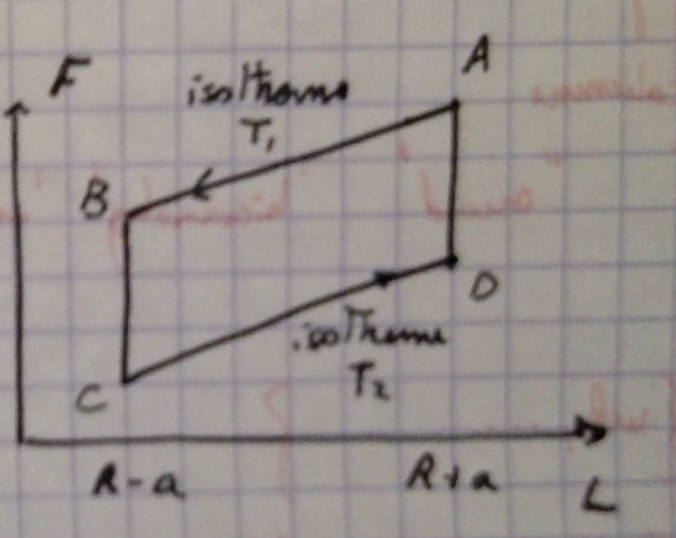
\includegraphics[width=0.4\linewidth]{thermo5.png}
\end{figure}	
Les transformations $AB$ et $CD$ sont des isothermes et $BC$ et $DA$ sont des iso-longueur.

\item[•] Pour trouver les expressions du travail (échange mécanique) et de la quantité chaleur reçue (échange thermique) sur une transformation, il faut appliquer le premier principe au 4 étapes du cycle, par exemple pour la transformation $AB$ : $\Delta U_A^B = W_A^B + Q_A^B$. 

Le travail se calcul grâce à $W_A^B=\int_{R+a}^{R-A}dL F$, puis la chaleur $Q_A^B$ se déduit de l'expression de $\Delta U_A^B$ avec l'équation de premier principe. 

\subsubsection*{Transformation AB}
Pour le travail, on oublie pas de faire un dl à l'ordre 1 en $a$.
\begin{equation}
W_A^B=\int_{R+a}^{R-a}dL F = \int_{R+a}^{R-A}dL =-2a\left( F_0-\sigma(T_1-T_0)  \right) -2a\rho(R-L_0)
\end{equation}

Énergie interne, toujours avec un dl en $a$ : 
$\Delta U_A^B = -2a(F_0-\sigma T_0)-2a\rho(R-L_0)$

Donc la chaleur est $Q_A^B=\Delta U_A^B-W_A^B=-2a\sigma T_1$

\subsubsection*{Transformation BC}
Il n'y a pas de travail car pas de variation de longueur.

L'énergie interne est : $\Delta U_B^C=C_L(T_2-T_1)$

La quantité de chaleur est donc : $Q_B^C=\Delta U_B^C = C_L(T_2-T_1)$

\subsubsection*{Transformation CD}
Il suffit de remplacer $a\longleftarrow -a$ et $T_1\longleftarrow T_2$ pour les différents calculs de la transformation $AB$.

Travail :
\begin{equation}
W_C^D=\int_{R-a}^{R+a}dL F = \int_{R+a}^{R-A}dL =2a\left( F_0-\sigma(T_2-T_0)  \right) +2a\rho(R-L_0)
\end{equation}

Énergie interne : $\Delta U_C^D = 2a(F_0-\sigma T_0)+2a\rho(R-L_0)$

Quantité de chaleur : $Q_C^D=2a\sigma T_2$

\subsubsection*{Transformation DA}
Il n'y a pas de travail car pas de variation de longueur.

L'énergie interne est : $\Delta U_D^A=C_L(T_1-T_2)$

La quantité de chaleur est donc : $Q_D^A=\Delta U_D^A = C_L(T_1-T_2)$

\subsubsection*{Bilan}
Au final, sur le cycle : 
$W=2a\sigma(T_2-T_1)$, $Q=2a\sigma(T_2-T_1)$ et $\Delta U=0$.

\item[•]
Le travail est moteur car $W<0$. Il faut bien noter que le sens est inversé par rapport à un diagramme "classique" car ici $\delta W = +FdL$ et non $\delta W = - pdV$.

\item[•]

Le rendement peut être alors défini comme : $\eta = \frac{-W}{Q_A^B + Q_D^A}$, car le fil reçoit de la chaleur par la source chaude pendant les transformations $AB$ et $DA$.

Alors on trouve :
\begin{equation}
\eta = \frac{2a\sigma(T_1-T_2)}{2a\sigma T_1+C_L(T_1-T_2)}
\end{equation}

\end{itemize}

\section*{Exercice 6}

\begin{itemize}
\item[•] Le système à définir est l'ensemble de la masse $M$, du piston et du gaz parfait contenu dans le cylindre. Son énergie totale $E$ s'écrit alors :$E = E_c + E_{pot} + U$. On s'intéresse à la situation $1$ (avant le lâcher de la masse) et à la situation 2 (après le lâcher de la masse, à l'équilibre).

L'énergie cinétique est nulle pour ces situations car on est à l'équilibre. 

Le premier principe s'écrit alors : $\Delta E_{pot} +\Delta U = W + Q$

Comme la paroi est adiabatique, $Q$ est forcément nul. La pression extérieure étant constante et égale à $P_0$, il s'écrit : $W=-P_0(V_2-V_1)=-P_0S(x-a)$, si $x$ est la hauteur finale du piston.

Comme le gaz est parfait, $\Delta U = c_V(T_2-T_1)$.

On a donc :
\begin{equation}
	c_V(T_2-T_1) + mg(x-a) + Mg(x-a-H)=-P_0S(x-a)
\end{equation}
On a supposé que la variation d'énergie potentiel du gaz était négligeable. 

Comme le gaz est parfait, 
\begin{equation}
c_VT_1=\frac{nRT_1}{\gamma-1}=\frac{P_1Sa}{\gamma-1}=\frac{P_0Sa+mga}{\gamma-1}
\end{equation}
En utilisant la relation des pressions à l'équilibre : $P_1=P_0+mg/S$.

De même : $c_VT_2=\frac{P_0Sa+(m+M)gx}{\gamma-1}$.
On obtient donc à la fin :
\begin{equation}
	(P_0S+(m+M)g)x = \frac{\gamma-1}{\gamma}Mg(a+H)+(P_0S+mg)Sa
\end{equation}

\item[•] Pour retrouver $x=a$, il suffit juste résoudre l'équation en $H$ précédente si $x=a$. On trouve :
\begin{equation}
	H_C=\frac{a}{\gamma-1}
\end{equation}

\end{itemize}

\section*{Exercice 7}

\begin{itemize}
	\item[•] Le gaz fuit dans $A$. Le piston avance jusqu'à être en équilibre de pression ($V_A<V_C$) ou s'écrase contre la paroi ($V_A>V_C$).
	\item[•] On commence par calculer le travail reçu par le gaz dans le volume $B$. Comme la pression est constante : 
	
	$W = -P_0\int_1^2 dV_{balayé}=P_0(V_A+V_B-V_1)$, où$V_1$ est le volume final du gaz. 
	
	L'état final sera totalement décrit par les variables d'état $T_1$ et $P_1$. En appliquant le premier principe sur le système {A + B} (y compris le vide initial dans $A$), on obtient : 
	$\Delta U = nc_V(T_1-T_0) = W$ car il n'y a pas d'échange de chaleur avec l'extérieur. Alors :
	
\begin{equation}
	\frac{R}{\gamma-1}(T_1-T_0)=P_0(V_A+V_B-V_1)
\end{equation}
cad :
\begin{equation}
	\frac{R}{\gamma-1}(P_0V_1-P_0V_A)=P_0(V_A+V_B-V_1)
\end{equation} 

\noindent\fbox{\parbox{\linewidth-2\fboxrule-2\fboxsep}{
On trouve alors : $V_1=V_A+\frac{\gamma-1}{\gamma}V_B$ et $T_1=\frac{P_0V_1}{R}=\frac{P_0}{R}\left(  V_A+\frac{\gamma-1}{\gamma}V_B\right) $
}}

Dans le cas décrit, $V_1>V_B$. Le cas limite est lorsque $V_1=V_B=V_C$ cad $ V_C=\gamma V_A$

\item[•] La variation d'entropie s'écrit $\Delta S = S_e + S_c$.
Or $\Delta S = nc_p\ln\frac{T_1}{T_0} - nR\ln\frac{P_1}{P_0}$. Comme $P_0=P_1$ :

\noindent\fbox{\parbox{\linewidth-2\fboxrule-2\fboxsep}{
\begin{equation}
	\Delta S = \frac{\gamma R}{\gamma - 1}\ln\left(\frac{T_1}{T_0} \right) =\frac{\gamma R}{\gamma-1}\ln \left( 1+\frac{(\gamma-1)V_B}{\gamma V_A}\right) 
\end{equation}
}}

On a bien $\Delta S =S_c>0$ ($S_e=0$ car il n'y a pas d'échanges avec l'extérieur.

\item[•] Si $V_A>V_C$, à l'état final on a $V_A=V_1$. L'état final est donc déterminé par la pression $P_1$.

Le premier principe donne : $\frac{R}{\gamma-1}(T_1-T_0)=P_0V_A$
Avec la loi des gaz parfaits, on trouve :

\noindent\fbox{\parbox{\linewidth-2\fboxrule-2\fboxsep}{
\begin{equation}
	P_1=\frac{\gamma P_0V_A}{V_B}
\end{equation}
}}

\end{itemize}

\end{document}
